\section{Bluetooth}

\begin{frame}[t]
	\frametitle{Bluetooth}

	\begin{minipage}[t]{0.50\linewidth}
		\begin{block}{Historique}
			\begin{itemize}
				\item 1994 : Création
				\item 1998 : SIG
				\item 1999 : 1.0
				\item 2004 : 2.0 BR / EDR
				\item 2010 : 4.0 BLE
				\item 2014 : 4.2
			\end{itemize}
		\end{block}
	\end{minipage}
	\begin{minipage}[t]{0.25\linewidth}
		\begin{figure}
			
\includegraphics[height=2.5cm]{img/bt_logo.png}
		\end{figure}
	\end{minipage}
\end{frame}

\begin{frame}
	\frametitle{Standard Bluetooth}
	\center{\textbf{Services}, \textbf{Profils} et \textbf{Protocoles}}
	\vspace{0.5cm}
	\begin{itemize}
		\item Liaison physique
		\item Adressage physique
		\item Controle de flux
		\item Multiplexage
		\item Chiffrement
		\item Protocoles over Bluetooth
		\item "Profils"
	\end{itemize}
	\vspace{0.5cm}
	\tiny{\url{https://www.bluetooth.com/specifications/adopted-specifications}}
\end{frame}

\begin{frame}
	\frametitle{Dénomination}

	\begin{minipage}[t]{0.30\linewidth}
		\begin{block}{Classique}
			\begin{itemize}
				\item Classique
				\item BR/EDR
				\item 2.0 3.0 3.1
				\item Bluetooth
			\end{itemize}
		\end{block}
		\begin{figure}
			
\includegraphics[width=\linewidth]{img/Bluetooth_Logo.png}
		\end{figure}
	\end{minipage}
	\begin{minipage}[t]{0.30\linewidth}
		\begin{block}{Les deux}
			\begin{itemize}
				\item Dual mode
				\item Smart Ready
				\item 4.0 4.1 4.2
			\end{itemize}
		\end{block}
		\begin{figure}
			
\includegraphics[width=\linewidth]{img/Bluetooth_Smart_Ready_Logo.jpg}
		\end{figure}
	\end{minipage}
	\begin{minipage}[t]{0.30\linewidth}
		\begin{block}{Low Energy}
			\begin{itemize}
				\item Low Energy
				\item Smart
				\item Wibree
				\item 4.0 4.1 4.2
			\end{itemize}
		\end{block}
		\begin{figure}
			
\includegraphics[width=\linewidth]{img/Bluetooth_Smart_Logo.png}
		\end{figure}
	\end{minipage}
\end{frame}


\begin{frame}
	\frametitle{Architecture physique}
	\begin{block}{Host et controller séparés}
		\begin{minipage}[t]{0.48\linewidth}
		\begin{figure}
			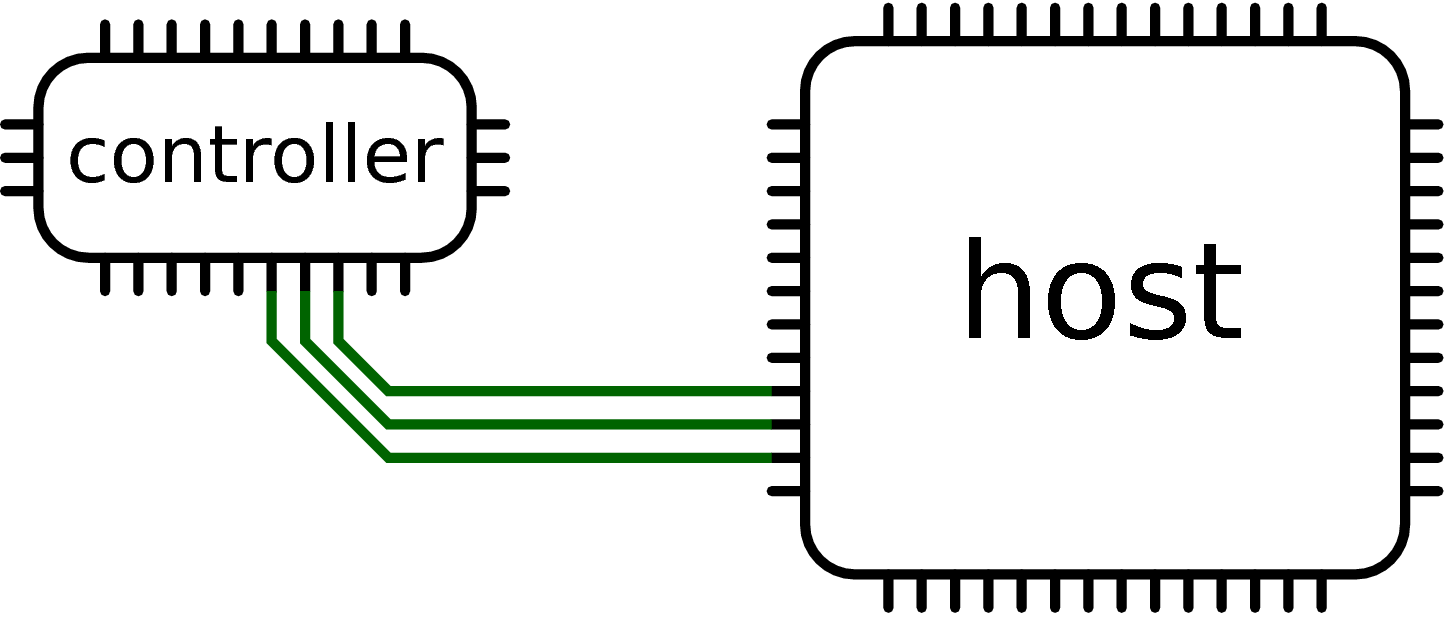
\includegraphics[width=4cm]{img/HC_sep.png}
		\end{figure}
		\end{minipage}
		\begin{minipage}[t]{0.48\linewidth}
		\begin{figure}
			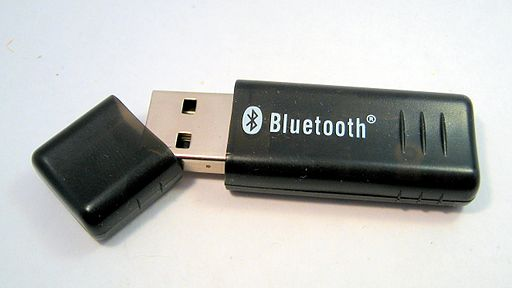
\includegraphics[width=3cm]{img/dongle.jpg}
		\end{figure}
		\end{minipage}
	\end{block}
	\begin{block}{System on a Chip}
		\begin{minipage}[t]{0.48\linewidth}
		\begin{figure}
			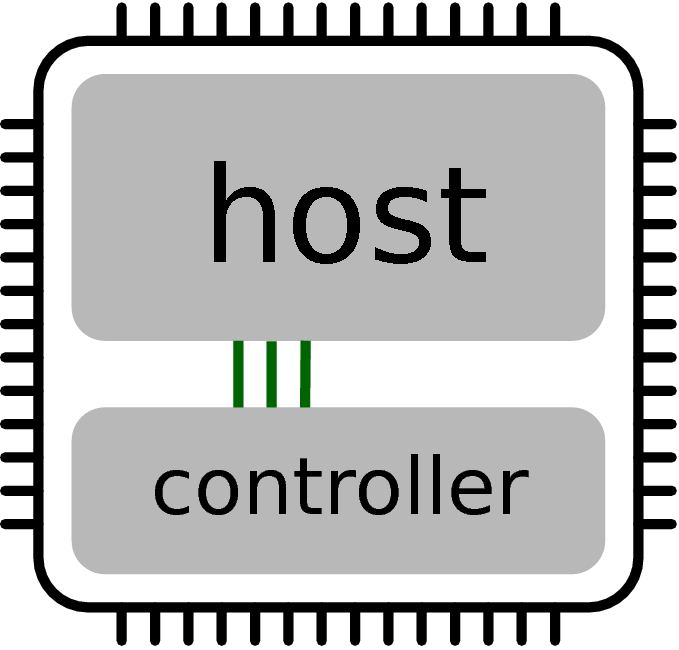
\includegraphics[width=2cm]{img/HC_soc.png}
		\end{figure}
		\end{minipage}
		\begin{minipage}[t]{0.48\linewidth}
		\begin{figure}
			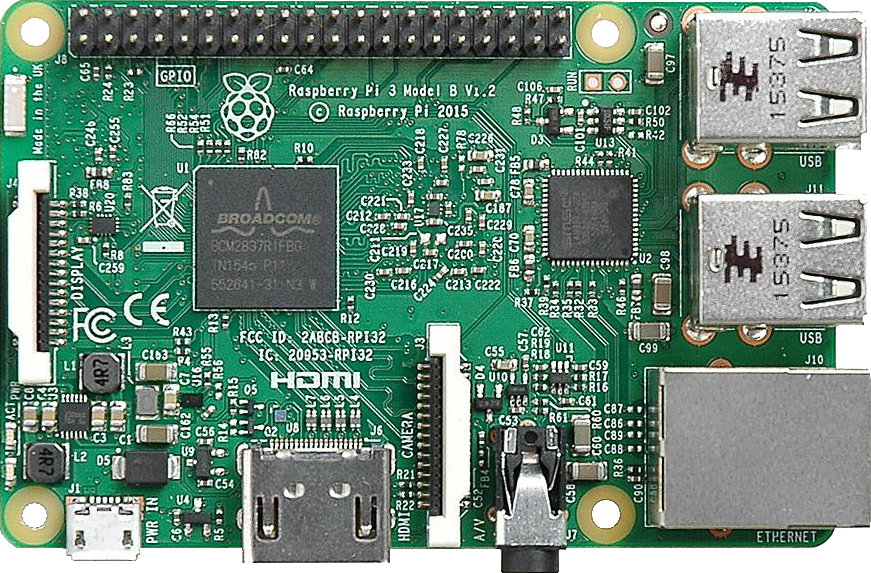
\includegraphics[width=3cm]{img/rpi3.png}
		\end{figure}
		\end{minipage}
	\end{block}
\end{frame}


\begin{frame}[t]
	\frametitle{Bluetooth Classique}
	\begin{minipage}[t]{0.30\linewidth}
		\vspace{0.5cm}
		\begin{block}{Radio}
			\begin{itemize}
				\item 2.4 GHZ
				\item 79 canaux
				\item FHSS
			\end{itemize}
		\end{block}
	\end{minipage}
	\begin{minipage}[t]{0.66\linewidth}
		\vspace{0.5cm}
		\center{\Large{Profils}}
		\vspace{0.5cm}
		\begin{itemize}
			\item Audio
			\item Transfert de fichiers
			\item IP / LAN
			\item Port série
			\item Partage de contacts
			\item Human Interface Device
			\item Découverte de services
		\end{itemize}
	\end{minipage}
\end{frame}

\begin{frame}
	\frametitle{Architecture logique}
	\begin{minipage}{0.45\linewidth}
		\begin{figure}
			\includegraphics[height=6cm]{img/HCI.png}
		\end{figure}
	\end{minipage}
	\begin{minipage}{0.50\linewidth}
		\begin{block}{Host}
			\begin{itemize}
				\item Profils et applications
				\item Différents protocoles
				\item Abstraction
				\item Multiplexage
			\end{itemize}
		\end{block}
		\begin{block}{Controller}
			\begin{itemize}
				\item Chiffrement
				\item Connexion
				\item Transmission physique
			\end{itemize}
		\end{block}
	\end{minipage}
\end{frame}

